\documentclass{article}
\usepackage{graphicx} % Required for inserting images
\usepackage{url}
\usepackage{hyperref}
\usepackage{biblatex} % Imports biblatex package
\usepackage{xpatch} % https://tex.stackexchange.com/questions/409297/why-are-my-notes-not-showing-while-using-apa-style-with-biblatex
\usepackage{filecontents}

\begin{filecontents}{FiveV2.bib}
@online{sengupta_survey_2020,
	title = {A {Survey} of {Moving} {Target} {Defenses} for {Network} {Security}},
	volume = {22},
	doi = {10.1109/COMST.2020.2982955},
	number = {3},
	journal = {IEEE Communications Surveys \& Tutorials},
	author = {Sengupta, Sailik and Chowdhary, Ankur and Sabur, Abdulhakim and Alshamrani, Adel and Huang, Dijiang and Kambhampati, Subbarao},
	year = {2020},
	pages = {1909--1941},
	note = {},
}

@online{guo_survey_2022,
	title = {A {Survey} on {Space}-{Air}-{Ground}-{Sea} {Integrated} {Network} {Security} in {6G}},
	volume = {24},
	doi = {10.1109/COMST.2021.3131332},
	number = {1},
	journal = {IEEE Communications Surveys \& Tutorials},
	author = {Guo, Hongzhi and Li, Jingyi and Liu, Jiajia and Tian, Na and Kato, Nei},
	year = {2022},
	pages = {53--87},
	note = {},
}

@online{chen_empowering_2023,
	title = {Empowering {Network} {Security} {With} {Programmable} {Switches}: {A} {Comprehensive} {Survey}},
	volume = {25},
	doi = {10.1109/COMST.2023.3265984},
	number = {3},
	journal = {IEEE Communications Surveys \& Tutorials},
	author = {Chen, Xiang and Wu, Chunming and Liu, Xuan and Huang, Qun and Zhang, Dong and Zhou, Haifeng and Yang, Qiang and Khan, Muhammad Khurram},
	year = {2023},
	pages = {1653--1704},
	note = {},
}

@online{mao_security_2023,
	title = {Security and {Privacy} on {6G} {Network} {Edge}: {A} {Survey}},
	volume = {25},
	doi = {10.1109/COMST.2023.3244674},
	number = {2},
	journal = {IEEE Communications Surveys \& Tutorials},
	author = {Mao, Bomin and Liu, Jiajia and Wu, Yingying and Kato, Nei},
	year = {2023},
	pages = {1095--1127},
	note = {},
}

@online{he_survey_2020,
	title = {A {Survey} of {Privacy} {Protection} and {Network} {Security} in {User} {On}-{Demand} {Anonymous} {Communication}},
	volume = {8},
	doi = {10.1109/ACCESS.2020.2981517},
	journal = {IEEE Access},
	author = {He, Yun and Zhang, Min and Yang, Xiaolong and Luo, Jingtang and Chen, Yiming},
	year = {2020},
	pages = {54856--54871},
	note = {},
}
\end{filecontents}
\xpatchbibdriver{online}
{\printfield{entrysubtype}}
{\printfield{entrysubtype}%
\newunit\newblock
\printfield{note}}

\addbibresource{FiveV2.bib}

\title{Journal 3 (and survey paper search/review)}
\author{Christopher Colvin}
\date{September 10, 2023}

\begin{document}
\maketitle
\section{Get The Lay of The Land}
    \subsection{Initial Research Direction}
        \paragraph{I intend to search for network security based survey papers, with a focus on endpoint-based network security, or at least a centralized piece of equipment intended to address network security concerns of endpoints.}
    \subsection{Search For Survey Papers}
        \begin{enumerate}
            \item Navigated to
                \url{https://scholar.google.com/schhp?hl=en&as_sdt=0,6}
            \item Figure 1 shows the search settings in Google Scholar
                \begin{figure}[ht!] % source: https://tex.stackexchange.com/questions/550226/why-is-this-image-not-appearing-where-it-should-in-this-code
                \centering
                \caption{\label{fig:TableOfContentsSnippet.png}Screenshot of Google Scholar search settings.}
                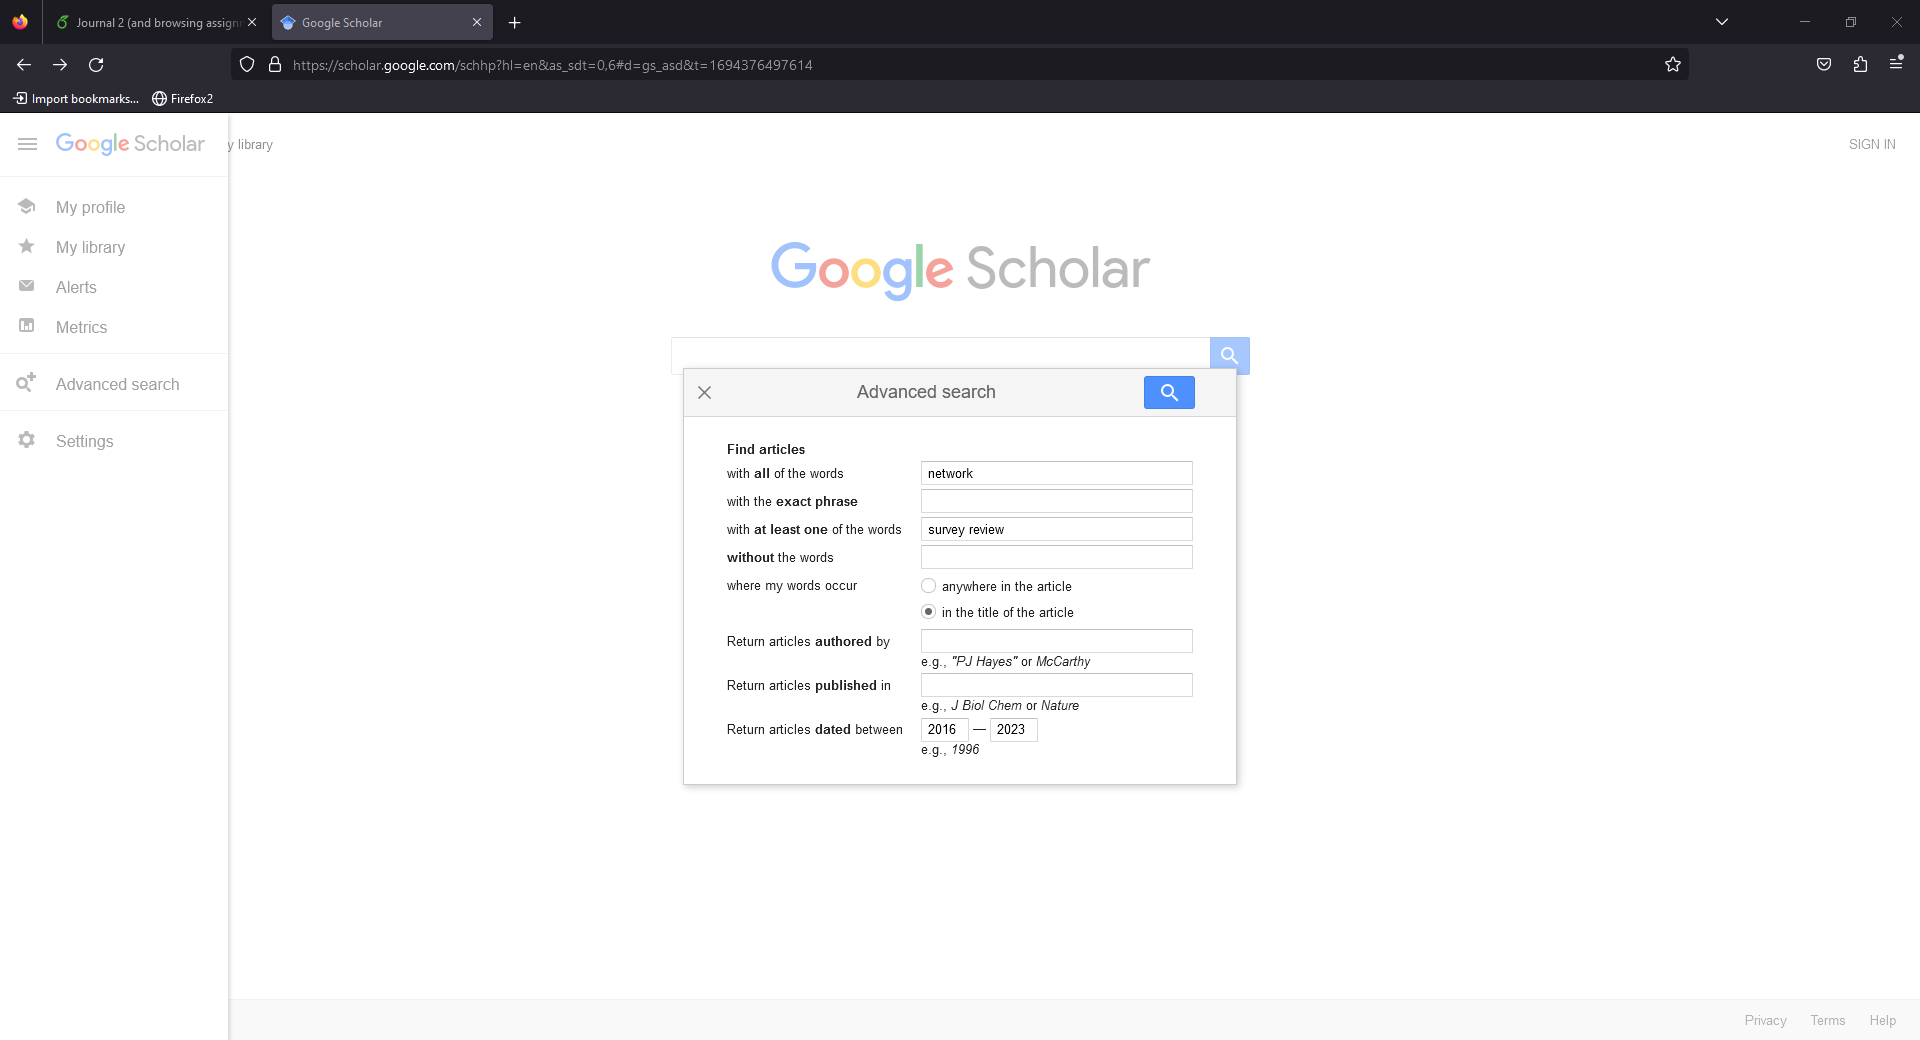
\includegraphics[width=0.89\textwidth, height=0.5\textwidth]{2023-09-10 14 18 04.png}
                \end{figure}
            \item This search provided little security papers, moving to include security
            \item Figure 2 shows the revised search settings in Google Scholar
                \begin{figure}[ht!] % source: https://tex.stackexchange.com/questions/550226/why-is-this-image-not-appearing-where-it-should-in-this-code
                \centering
                \caption{\label{fig:TableOfContentsSnippet.png}Screenshot of updated Google Scholar search settings.}
                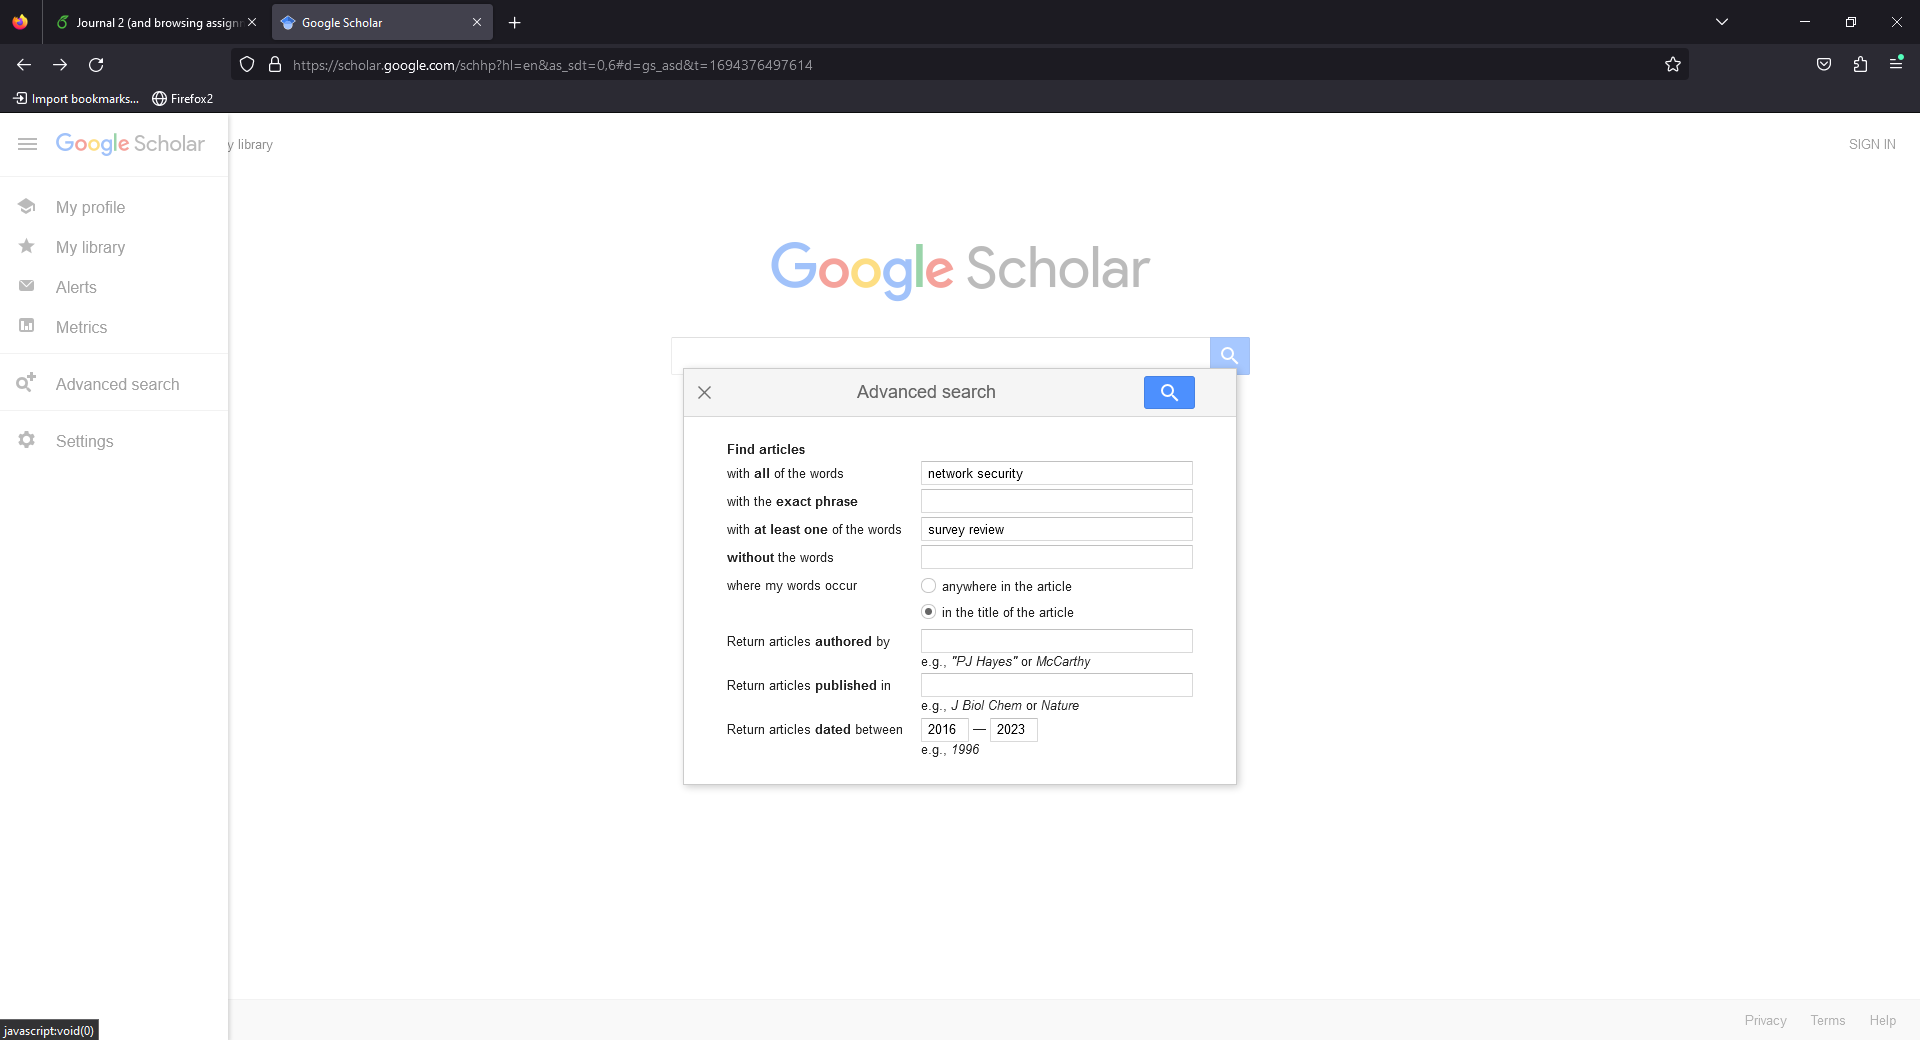
\includegraphics[width=0.89\textwidth, height=0.5\textwidth]{2023-09-10 14 20 09.png}
                \end{figure}
            \item Figure 3 shows the updated search had much better results 
                \begin{figure}[ht!] % source: https://tex.stackexchange.com/questions/550226/why-is-this-image-not-appearing-where-it-should-in-this-code
                \centering
                \caption{\label{fig:TableOfContentsSnippet.png}Screenshot of updated Google Scholar search results.}
                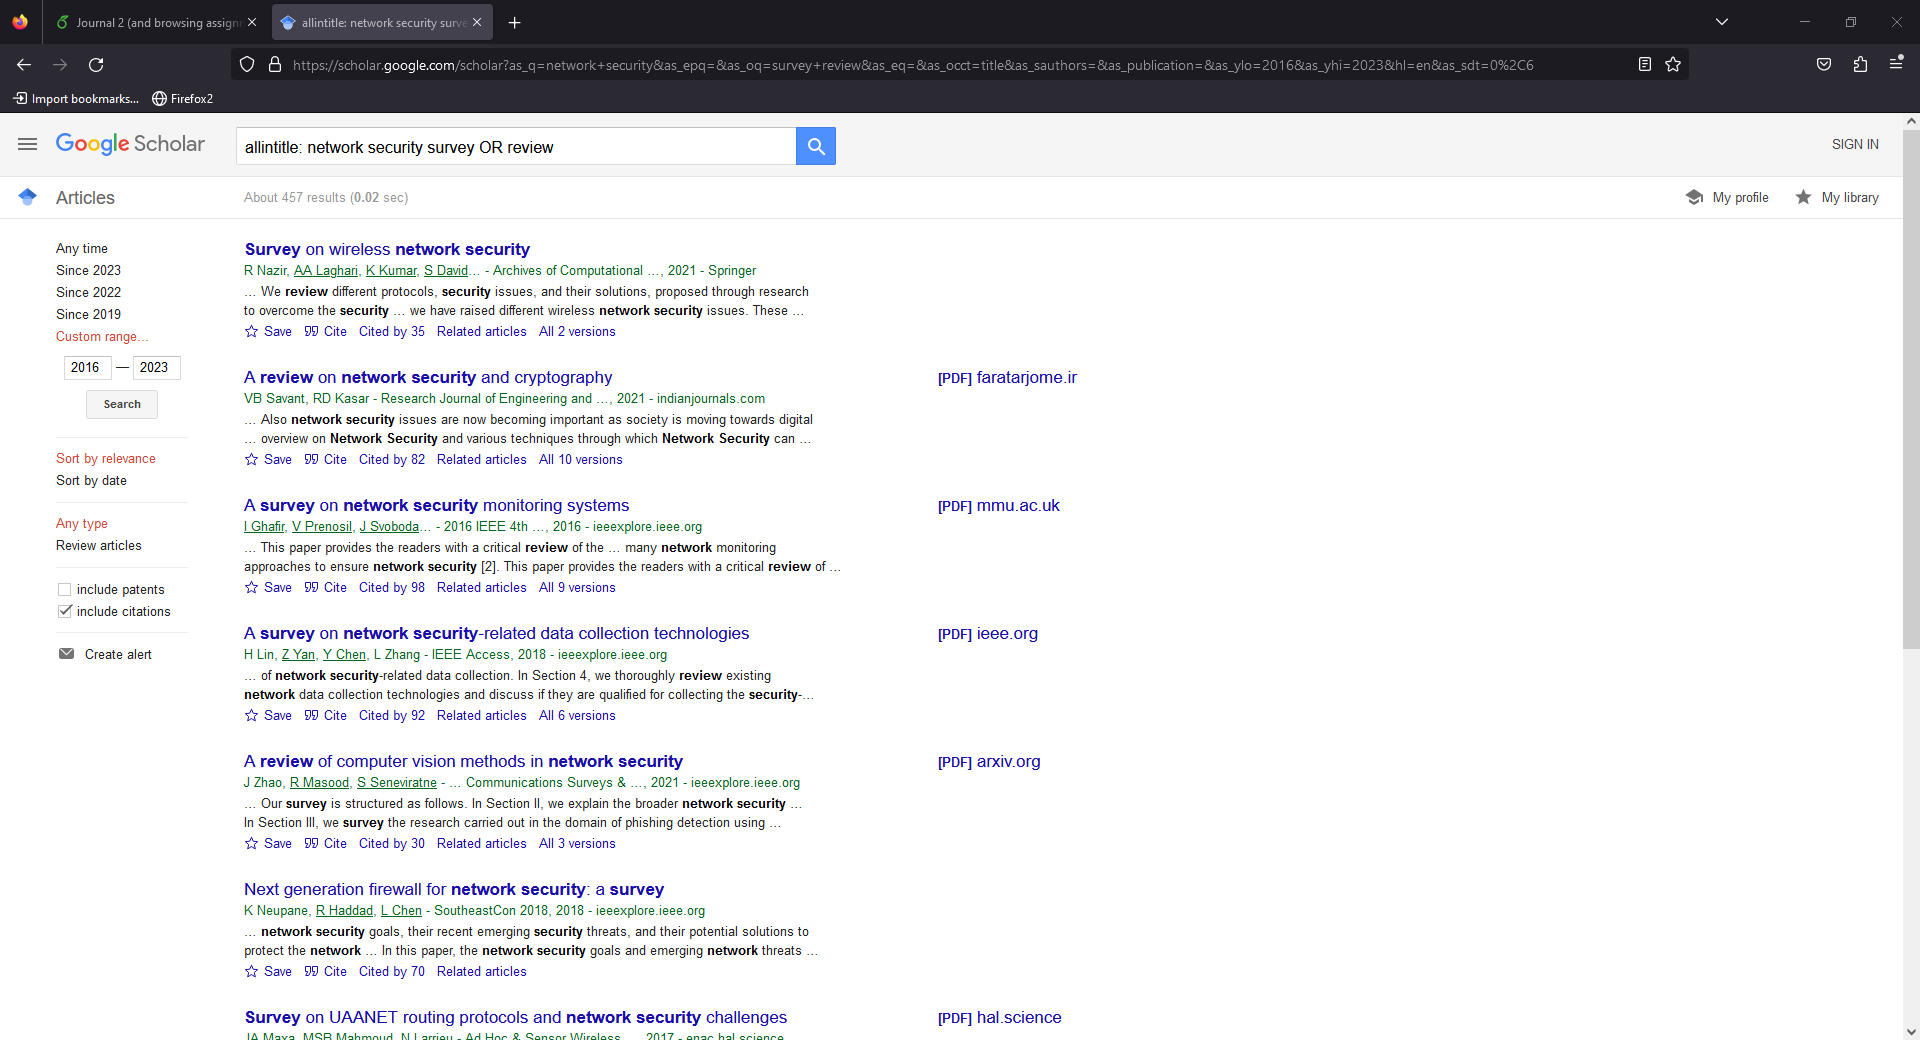
\includegraphics[width=0.89\textwidth, height=0.5\textwidth]{2023-09-10 14 24 37.png}
                \end{figure}
            \item Due to this search for survey papers resulting in less than 500 results, I am going to use a neat trick and will post the code here to perform analytics on the pages (in a fairly manual way instead of fully automoted, however still useful - without a web crawler on this search hyperlink for instance in Python and additional linux sort and awk commands)
            \item Figure 4 shows the result in Notepad++ (can use notepad qq in Linux as well). The first step is to build the raw amount of data and validate it is all there, I copied from each of the 45 pages @ up to 10 results per page to a text document, and counted the number of either ``Sign in" terms or ``PrivacyTermsHelp", as one of these occur on each page. The result is 45, I had to do this twice, because the robot popup messed up a page (htmlContentAndAppensions.txt).
                \begin{figure}[ht!] % source: https://tex.stackexchange.com/questions/550226/why-is-this-image-not-appearing-where-it-should-in-this-code
                \centering
                \caption{\label{fig:TableOfContentsSnippet.png}Screenshot of Notepad++ counting the sign in occurrences to confirm the number of pages.}
                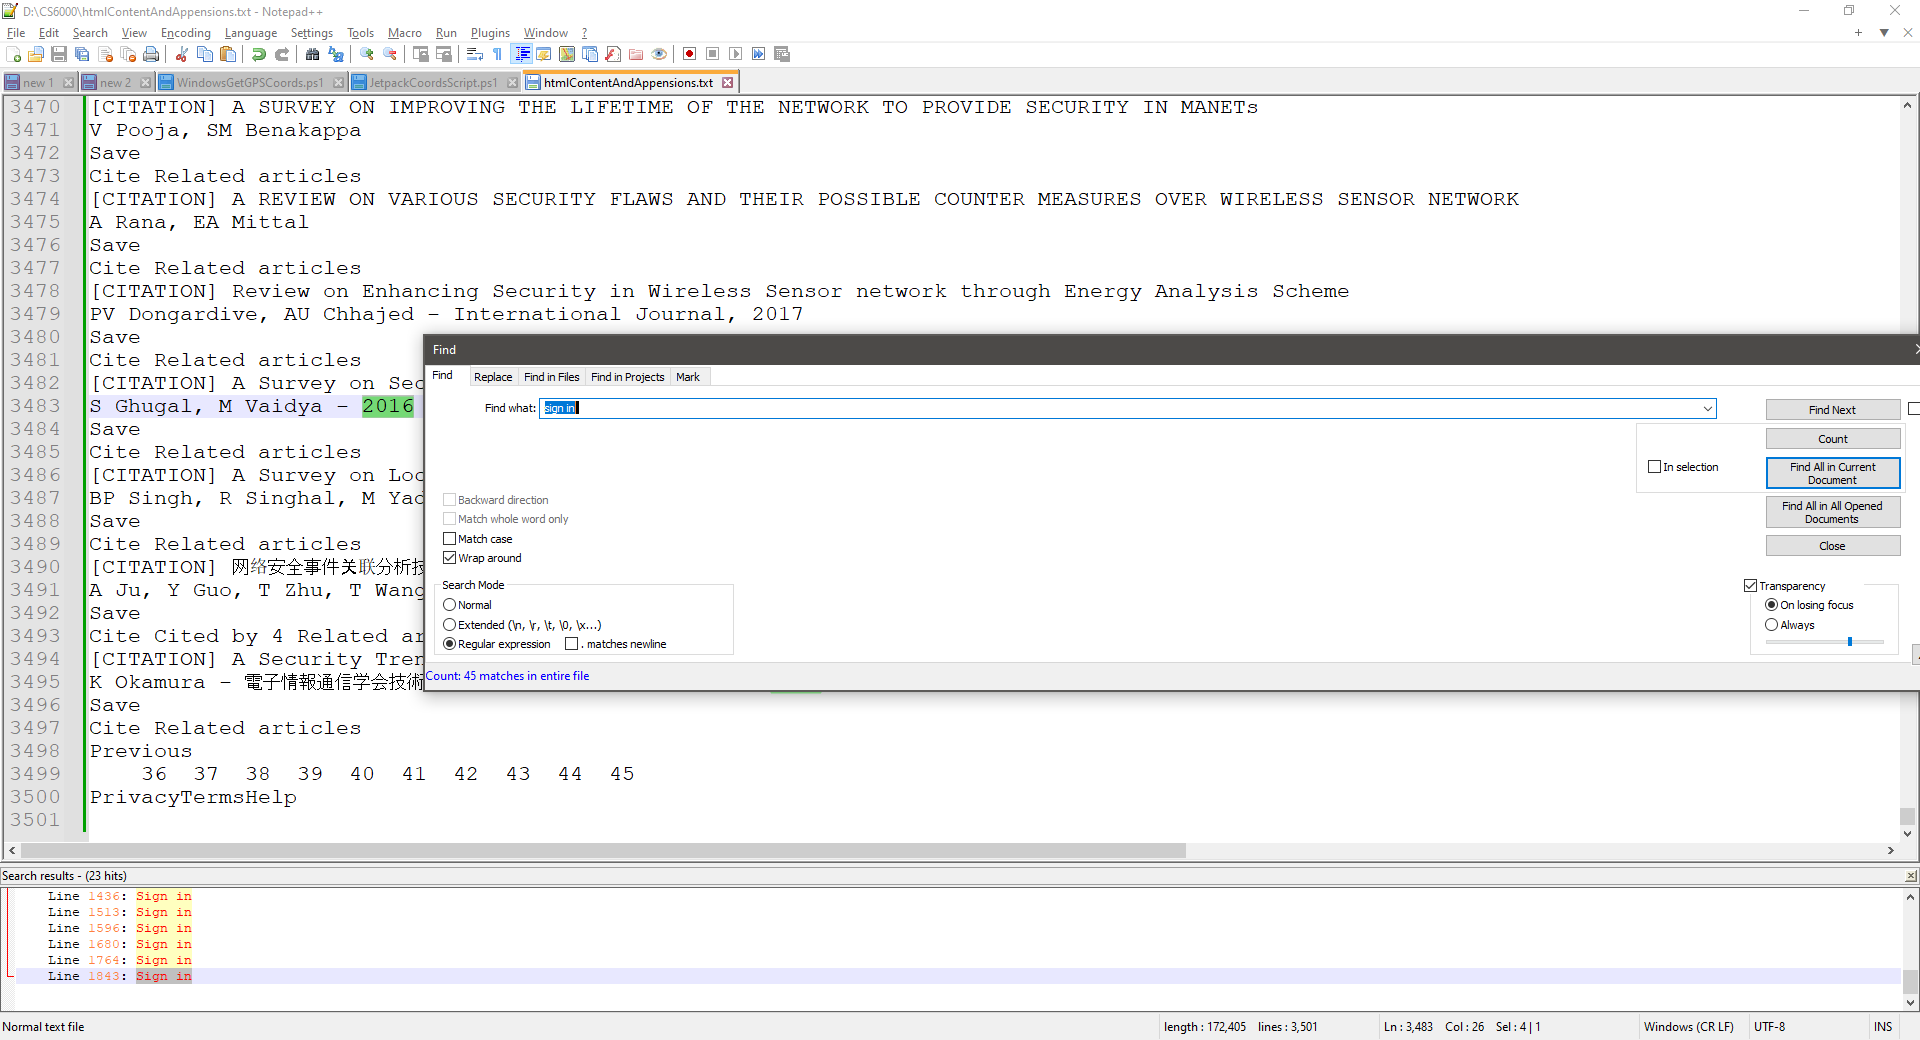
\includegraphics[width=0.89\textwidth, height=0.5\textwidth]{2023-09-10 15 08 52.png}
                \end{figure}
            \item I chose to use Ubuntu Desktop 22.04.1 using an old image ubuntu-22.04.1-desktop-amd64.iso, SHA256:c396e956a9f52c418397867d1ea5c0cf1a99a49dcf648b086d2fb762330cc88d, and use the prerequisites below to start the analytics
                \begin{enumerate}
                \item Install VMware Workstation Player (17.0.2 build-21581411 was on hand at the time)
                \item Download and Verify Ubuntu Desktop (22.04.1 was on hand at the time)
                \item Create a VM from ubuntu-22.04.1-desktop-amd64.iso
                \item Run and install Ubuntu Desktop
                \item Configure VMware settings to 4GB RAM and 2GB GPU memory
                \item Ensure network connectivity through terminal with the command ``ping google.com"
                \item Ensure network connectivity by using Mozilla Firefox to navigate to ``google.com"
                \item If successful, keep NAT settings, if not, choose Bridged and/or adjust firewalls
                \item In terminal run \[``sudo date -s ``\$(wget -qSO- --max-redirect=0 google.com 2>\&1 | grep Date: | cut -d' ' -f5-8)Z""\] to sync the Linux system time for updates to work
                \item In terminal run ``sudo apt update"
                \item In terminal run ``sudo apt full-upgrade"
                \item In terminal run ``sudo apt install libreoffice"
                \item In terminal run ``sudo apt install notepadqq"
                \item In terminal run ``sudo apt install pcregrep"
                \item In terminal run ``sudo apt install open-vm-tools"
                \end{enumerate}
            \item Figure 5 shows the resulting CSV in Ubuntu Desktop from a custom script being imported. Grep -E to discover the regular expression patterns, and sed -E to sanitize the data/inputs for a spreadsheet. Full log details in the attached Bash/Shell script file. Now the next step is to pull the results of this big set of data and build a spreadsheet for a reliable set of analysis. The spreadsheet allows for a dynamic use of the content by many (including my team working on a research proposal for example) on different operating systems, not just Linux, or a new script being needed for Windows. Whereas static Linux code to analyze this, would result in only Linux compatibility and a constant result, without the ability to rearrange, remove columns, or perform operations as such in a convenient (known) program such as MS Office Excel or LibreOffice Calc. This way it is collaborative and scalable with a team, regardless of technical experience as well.
                \begin{figure}[ht!] % source: https://tex.stackexchange.com/questions/550226/why-is-this-image-not-appearing-where-it-should-in-this-code
                \centering
                \caption{\label{fig:TableOfContentsSnippet.png}Screenshot of the importing of the analytics resulting CSV for sorting the cited by column.}
                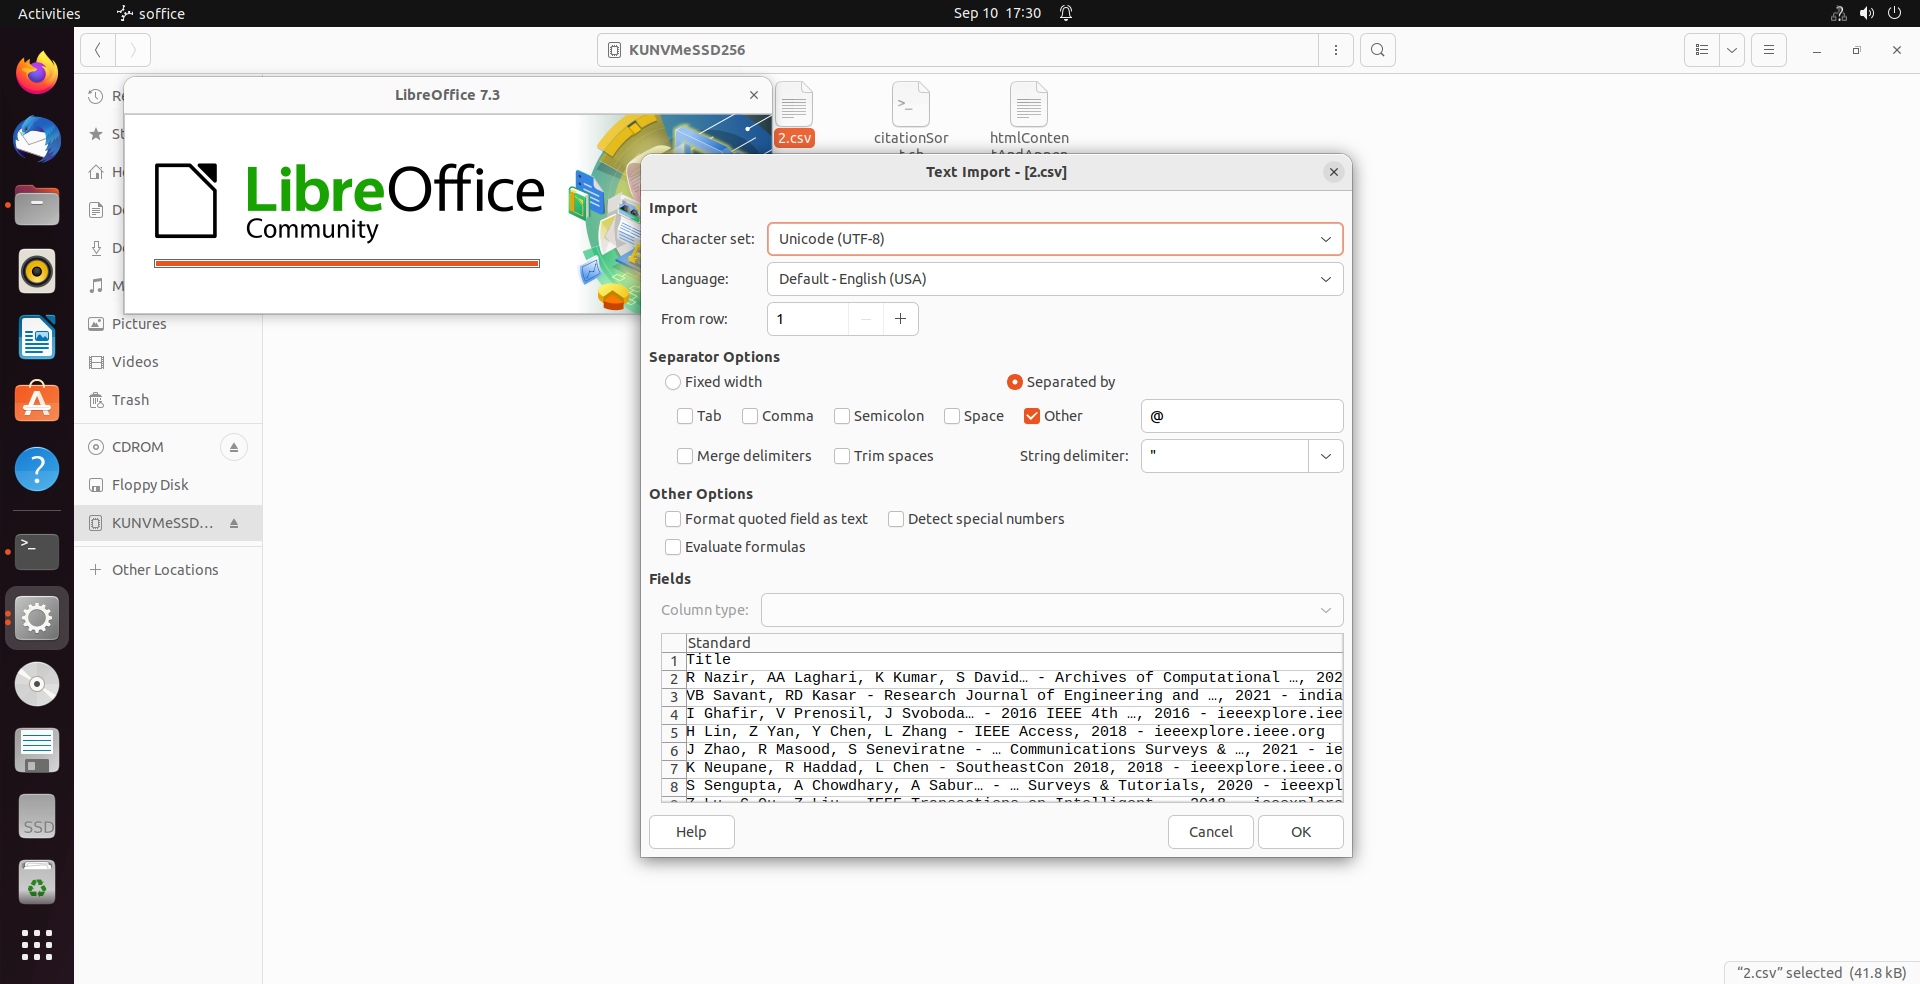
\includegraphics[width=0.89\textwidth, height=0.5\textwidth]{2023-09-10 17 31 03.png}
                \end{figure}
            \item Figure 6 shows LibreOffice and our analytics data now being visible and editable.
                \begin{figure}[ht!] % source: https://tex.stackexchange.com/questions/550226/why-is-this-image-not-appearing-where-it-should-in-this-code
                \centering
                \caption{\label{fig:TableOfContentsSnippet.png}Screenshot of the analytics data visible in LibreOffice Calc.}
                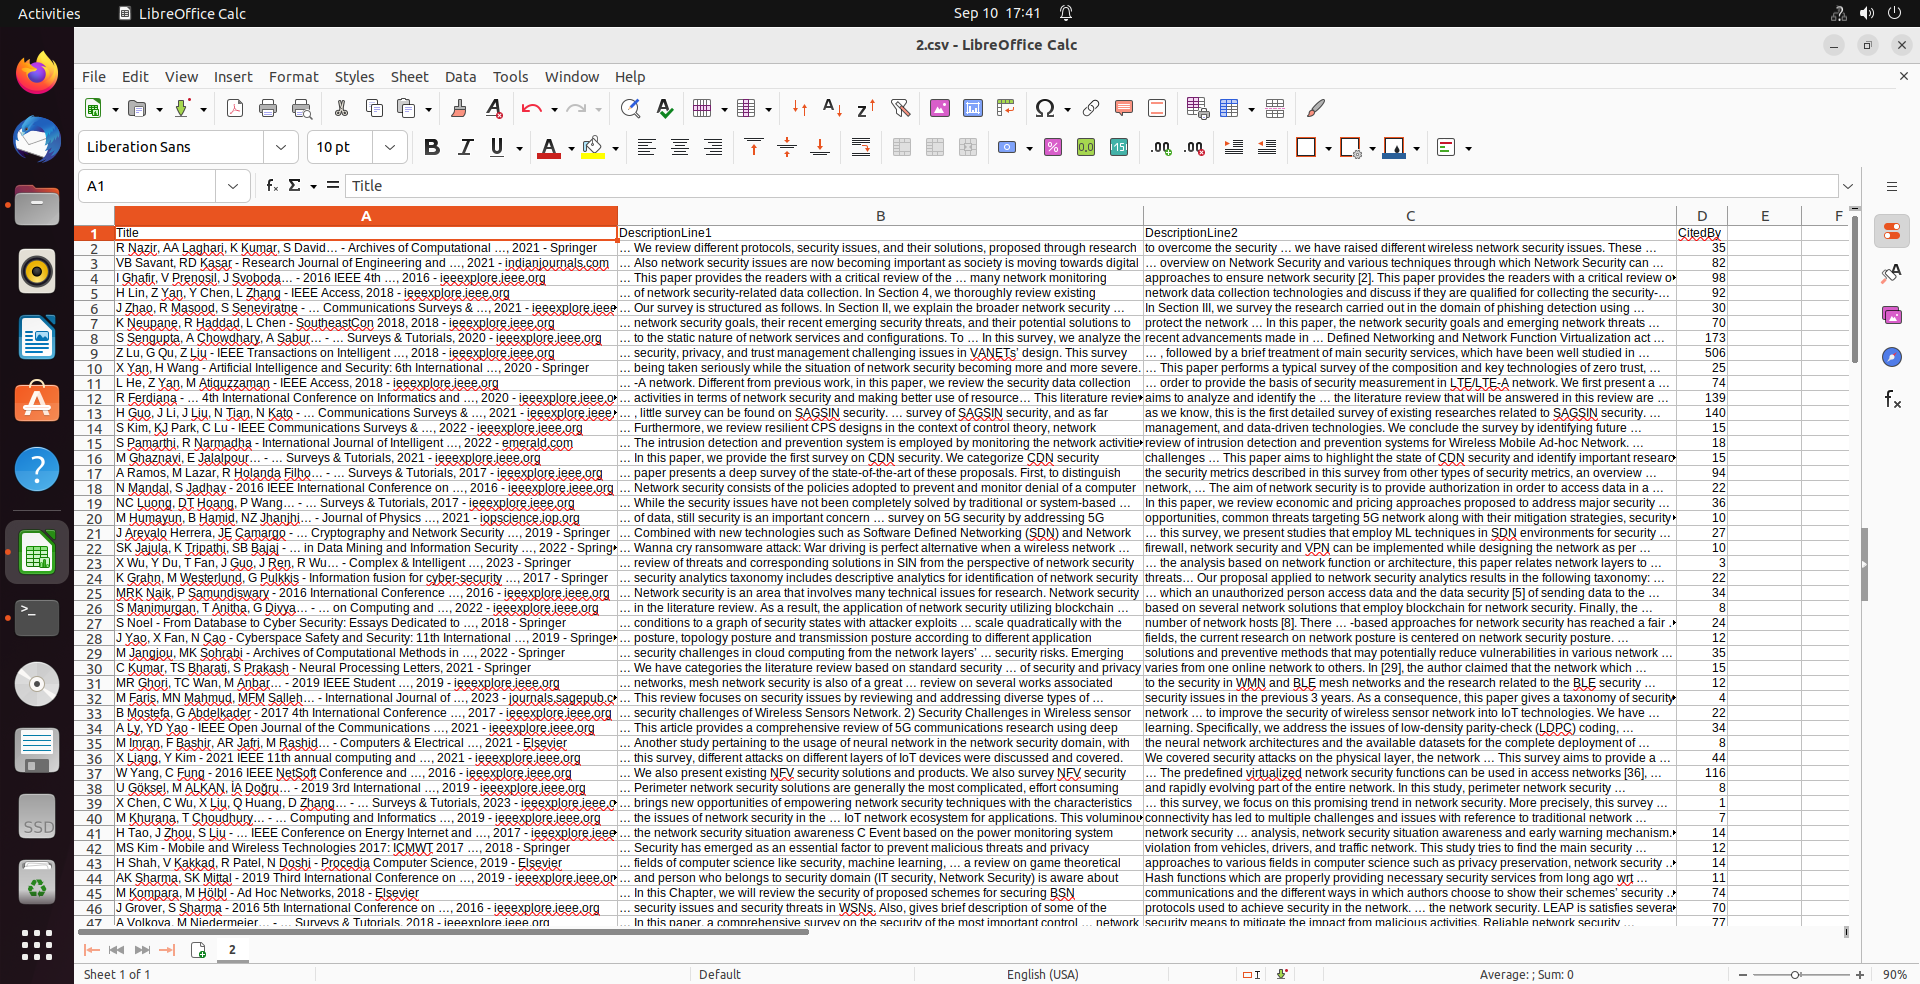
\includegraphics[width=0.89\textwidth, height=0.5\textwidth]{2023-09-10 17 41 42.png}
                \end{figure}
            \item Figure 7 shows AutoFilter and Bold text applied to the headers added from the script.
                \begin{figure}[ht!] % source: https://tex.stackexchange.com/questions/550226/why-is-this-image-not-appearing-where-it-should-in-this-code
                \centering
                \caption{\label{fig:TableOfContentsSnippet.png}Screenshot of our headers being bold and enabled with AutoFilter for sorting soon.}
                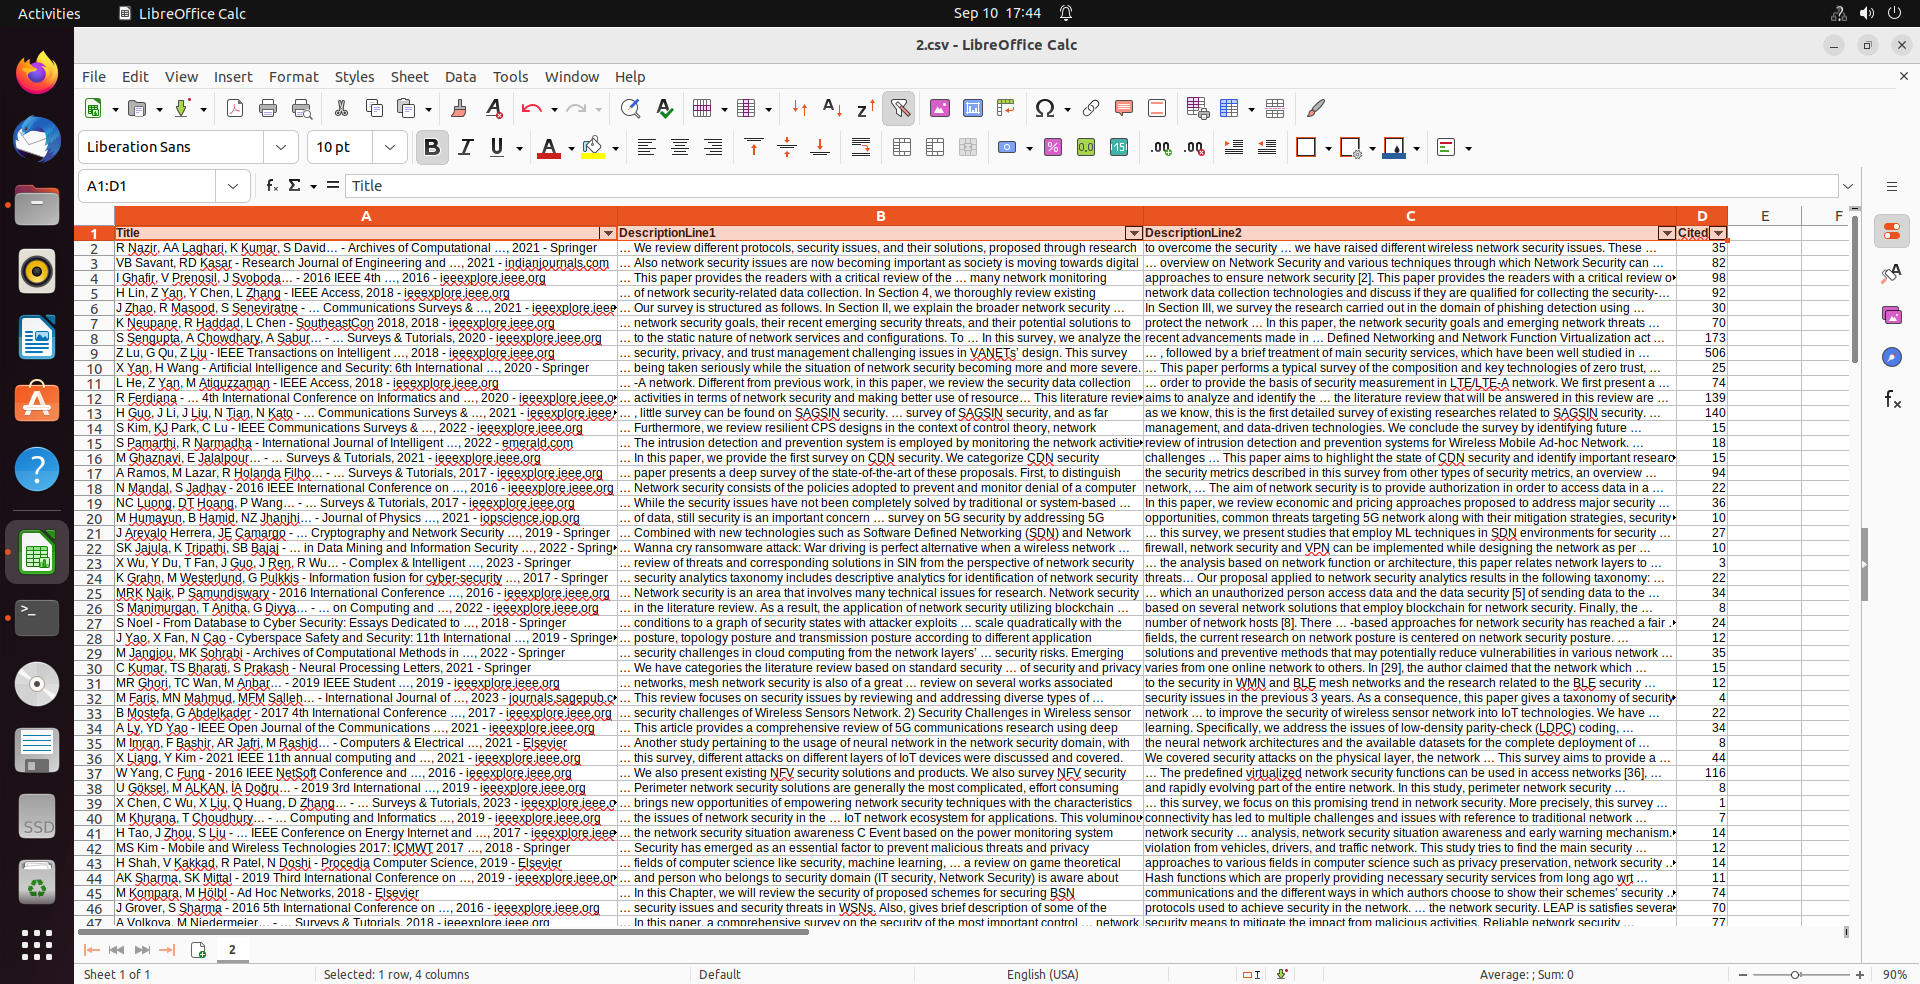
\includegraphics[width=0.89\textwidth, height=0.5\textwidth]{2023-09-10 17 44 56.png}
                \end{figure}
            \clearpage
            \item Figure 8 shows our Cited By column has been sorted in descending order. At this point is when I saved the spreadsheet visible in the screenshot as CSV, ODS, and XLSX to upload to the repo for review. At this point, I also noticed there are fewer papers here, the reason is some of the raw data contains Save and Cite Cited by content on the same line, not separate lines, my code only accounted for the separate line scenarios. For now, I am going to leave it as is, it reviewed a lot more papers than I was going to be able to recollect and save and analyze.
                \begin{figure}[ht!] % source: https://tex.stackexchange.com/questions/550226/why-is-this-image-not-appearing-where-it-should-in-this-code
                \centering
                \caption{\label{fig:TableOfContentsSnippet.png}Screenshot of our headers being bold and enabled with AutoFilter for sorting soon.}
                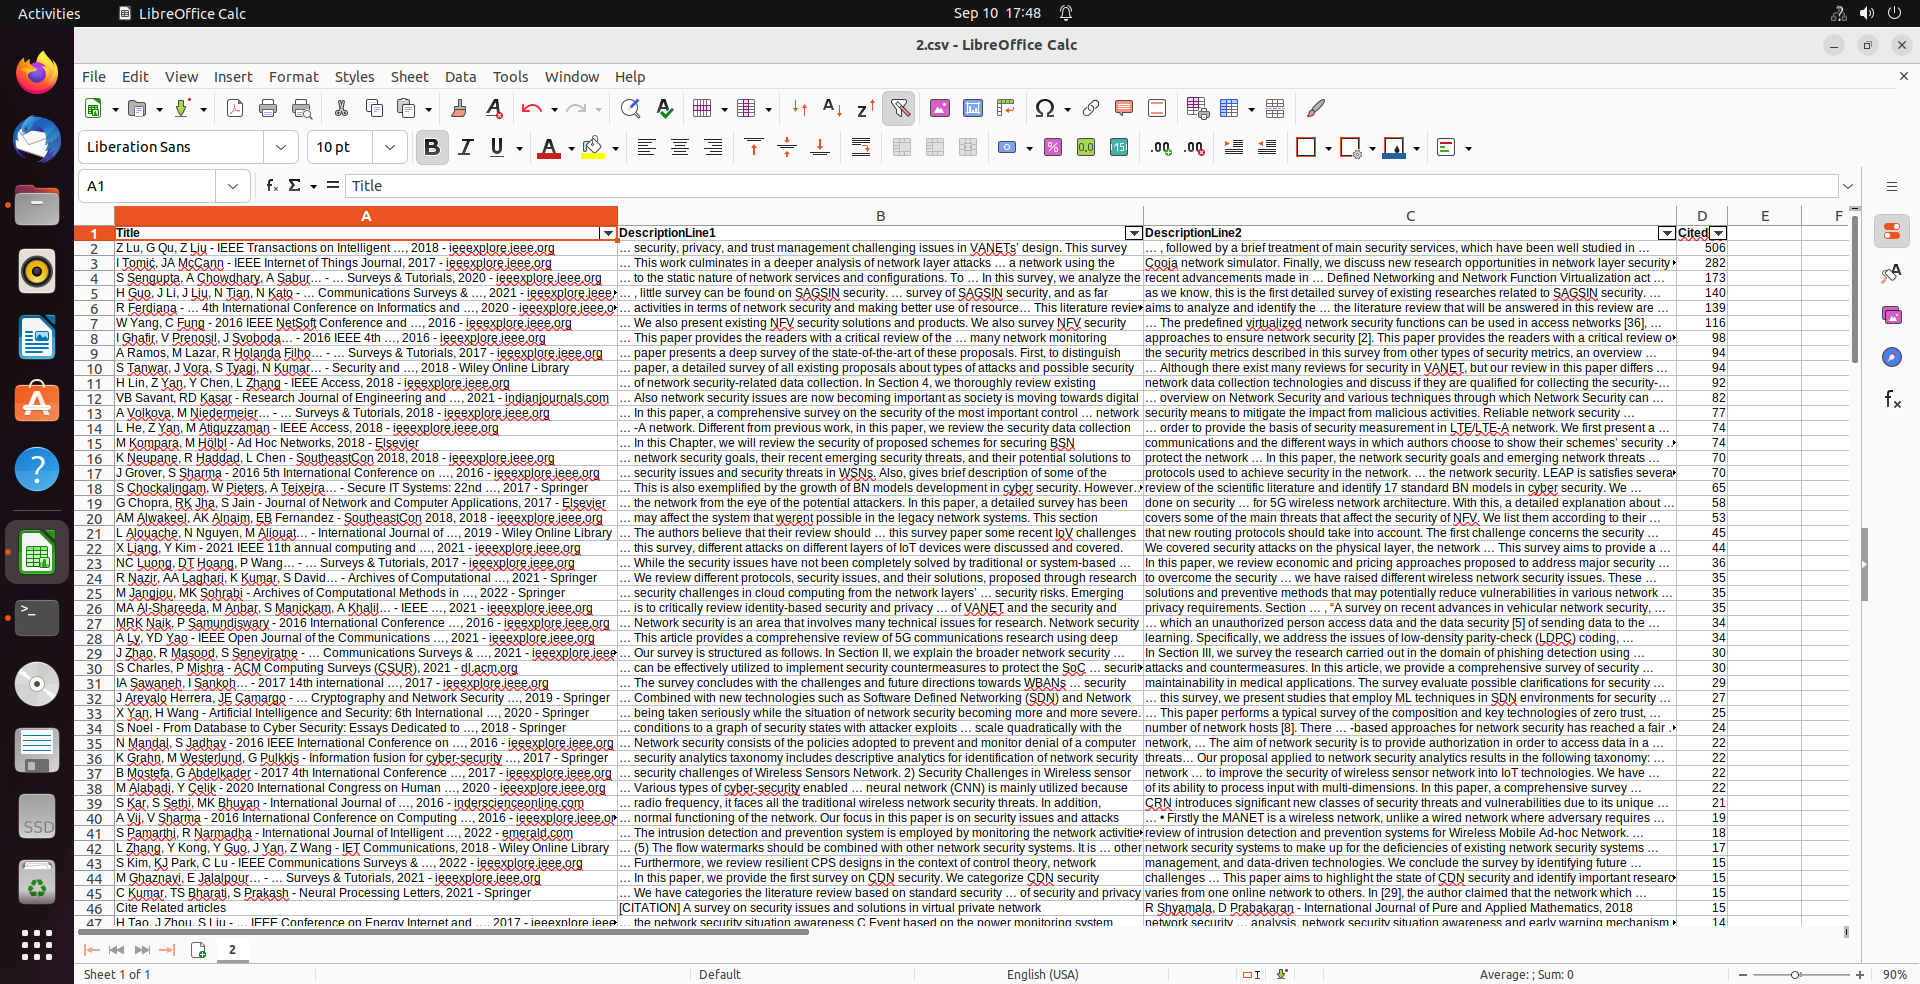
\includegraphics[width=0.89\textwidth, height=0.5\textwidth]{2023-09-10 17 48 14.png}
                \end{figure}
                \begin{enumerate}
                    \item[] Attachments for/from the analytics performed are below and attached
                    \item[] This attachment includes the content from each HTML page of the 457 results and the unfortunate oversight of Google Scholar having Save on the same line as the Cited by count
                    \item 0.txt
                    \item 1.txt
                    \item 2.csv (old, updated with an additional step for 3.csv, this was missing 104 cited by occurrences)
                    \item 2.txt (new, needed a new step to fix the 2.csv missing 104 cited by occurrences)
                    \item 2.ods
                    \item 2.xlsx
                    \item 3.csv (new, only missing 11 cited by occurrences)
                    \item 3.xlsx (new, only missing 11 cited by occurrences)
                    \item citationSort.sh (this is the newest version, missing 11 occurrences of cited by)
                    \item htmlContentAndAppensions.txt
                    \item There are still improvements to make to this analytics script, for instance the lines break when [CITATION] occurs, further debugging is required
                \end{enumerate}
            \item Our task, which I chose to accept, was to locate the most cited, and least cited relevant survey papers within 3 years. Using the analytics above resulted in a clear difference to assess the differences between the most and least cited papers.
            \item I decided to use the two most popular survey papers, one somewhere in the middle, and the two least popular survey papers, all from the last three years.
\end{enumerate}


    \subsection{Raw Notes From Critical/Creative Reads}
        \paragraph{
            \cite{sengupta_survey_2020}01/05. Top Cited. Time taken 44m15s. Critiqued. Raw notes follow the links below.
        }
        \hfill \break
        \href{
            https://ieeexplore.ieee.org/abstract/document/9047923
        }
            {A Survey of Moving Target Defenses for Network Security}
            \\
        \url{https://ieeexplore.ieee.org/abstract/document/9047923}
        \\\\
        \paragraph{ Perhaps we can share the analytics script with the class, and this is one option students can use to find their research interests, just a possibility.

The Good, The Bad, and The Defense, the way I like to present

The good, the network cloud infrastructures have become the go-to method for benefits in storage capacity and networking efficiency. The hook, what are we doing to secure it, are we doing enough? This is what they used in the paper, really good. The use of relying on, this is genius from a security standpoint, this paper is worded and structured to elicit a response from the audience that they are in danger, which acts as a story in a way to hook the reader, but it doesn’t push too hard by stating “you”, because that could offend those reading, excellent tense used.

Traditional, they set out what is being relied on currently with multiple shortcomings.
-Monitoring network traffic for malicious patterns
-Routinely patching known vulnerabilities
-Relying on the network perimeter defense such as Firewalls, Intrusion Detection Systems, Anti-malware tools
Are these enough to detect and thwart attacks?

First the attacker, with time on their side, recon, planning, this is the antagonist of the story, the protagonist has yet to be revealed. Second, these implementations are far from ideal in practice. The fear of Quality of Service (QoS) degradation, lastly Zero-day attacks, not exploits, not even reduced in the synonyms here. Really trying to elicit a response from the reader still.

Moving Target Defense (MTD) has emerged as a solution to proactively defend against adaptive adversaries, here is the protagonist at last, to save the day, it is a story.

Constantly move between multiple configurations, changing open ports, network configuration, running software, etc, diminishing the advantage of recon that the attacker inherently has against traditional defenses. It is clearly creatively resolving the conflict right before our eyes, and the language is an in-depth story now, it’s like we are entering chapter 2 very quickly and are relieved.

MTDs, even the attacker, with time on their side, will eventually predict this movement, thus, for MTDs, implicit randomness must be built in.

This survey categorizes MTDs based on what they shift, when they shift and how they shift. Chapter 3 begins.

Network Functions Virtualization, through VMs as defenses in containers that can be automated, reduced cost, and Software-Defined Networking (SDN) which enables technology for NFV, provides a centralized security policy enforcer. The language just keeps going, it is like an action film. Reinforcements have arrived, after Chapter 2 where the call to action was issued.

The key contributions of this survey are (1), (2), (3), (4). Very easy to critically read, this must contribute to the number of citations of this paper. (1) Umbrella to categorize MTD techniques proposed for network E> (2) Introduces a method to describe and understand assumptions and threat models of various MTDs, (3) gives overview of an MTD implemented defenses by researchers (this is a keyword here, it is speaking to the audience reading now, without stating you, or a specific job title, it is very well written). (4) how to evaluate an MTD qualitatively and quantitatively to measure the actual effectiveness with regards to security and performance.

The rest of the survey is organized in the following manner. In Section II, this is a story, this is using a tactic from the Bjork’s Desirable Difficulties (https://thelearnerlab.com/desirable-difficulties/) where they pretext the situation with a fill in the blank question. This is because they state, we introduce the reader to some background knowledge about the various stages of an attack in cloud systems, popular defenses etc., this is having the reader ask, what are the popular detections and defenses, as they state, without actually listing them here.

In this section (Section II), we discuss related surveys in the area of MTD that look at the aspects of characterizing and evaluating proactive defenses, this is another networking method for this paper to be popular, they are sharing the air with others in the field, and I expect they will appreciate the complement for their work being reference-able.

Related works and the need for this survey.

Most existing surveys only provide partial coverage relating to what, when, and how, which digs into the 7 Ws and is useful. This is applicable to move the elements of the network. Table I is awesome, of course with their survey coming in to fill in all of the personalized slots by the authors, very nice.

The novelty about the problem formulation is they have hooked the reader, and are now identifying the necessity to read the survey to implement the MTD properly, in other words, allowing the reader to save time by reading this paper.

I love all of the tables included, they truly have outdone themselves, this meets my expectations for a highly cited survey paper based on my analytics and impression. Very professional, well-planned and well-executed.

Very relevant to my research, because I have found 25 niche applications that can save even more resources and time than an entire MTD planning, design, implementation, and maintenance. I will try my best in the topic map as soon as possible, referencing parts of my research.

Command and Control is usually referred to as C2 if I am not mistaken, interesting choice for the acronym in this paper.

My research has been very people-system driven, it appears I will be more successful, as discussed in class, by relating my research applications to a company, agency, or broad scope to hook the reader and then get back to minutia of implementation, with figures and tables throughout.

The timing function, when to switch is definitely a part of my research, but more broad, and not as secure in my personal opinion, at this time. Game-based Security in SDN-enabled Cloud Networks.

Key Performance Indicators/Metrics, effective. Great summary.
44:15 time elapsed.}


        \paragraph{
            \cite{guo_survey_2022}02/05. Top Cited. Time taken 34m38s. Critiqued. Raw notes follow the links below.
        }
        \hfill \break
        \href{
            https://ieeexplore.ieee.org/abstract/document/9628162
        }
            {A Survey on Space-Air-Ground-Sea Integrated Network Security in 6G}
            \\
        \url{https://ieeexplore.ieee.org/abstract/document/9628162}
        \\\\
        \paragraph{ OSCAR being used here explicitly, the broad hook, ground network can no longer meet the requirements on network access at anytime and anywhere on the earth. Space-air-ground integrated network (SAGIN).

Not as prominent in the defined references. Very basic here.

A. Existing surveys. Current research is on single networks, or on the integration of different kinds of networks, satellite-ground and non-terrestial network. Security issues, Table I is quite effective, summarizes related surveys to SAGSIN security.

B. Motivation. Limitations of other surveys, single network segment in space or in the air, or on the integration of two-tiered segments like air-ground network, sateelite-terrestrial network, etc. UAVs can relay between ground and satellite network transmission. This can reduce ground radio jamming and improve performance, however it is possible to attack satellites or UAVs through the transmissions themselves. The open security of UAV links allows for jamming, eavesdropping, and injection of false commands to satellites. We need to consider the uniqueness of a hybrid network, and design new secure group communication protocols. This may be a new unforeseen circumstance for the application of my network security research, it is not just about encryption, but the devices transmitting and receiving, I can bypass many of these security threats by using my encapsulation through other protocols and custom header information as a few tactics to leverage. My cryptography research could also address this concern of encryption to speed penalty they experience in UAVs.

C. Contributions. This survey contributes in the following ways. 

Background section is kind of interesting, not as appealing to myself. Time-variability has been one of the greatest strengths present in all of my forensics experience with cellular networks. Change of relative distance between nodes, transmission delay, or handover between nodes for network structure and affect the routing of local nodes, leading to performance impact on aspects of the previous and new networks. My research could be adapted to include such a change effectively and proactively resolve these performance issues as well.

Not disagreement with E. Challenges.

4) Security: A four-layer heterogeneous network, open links and dynamic topologies. DoS, jamming, spoofing, unauthorized access, malware, this is normal.

Section IV, security threats in SAGSIN, great categorization, lots of separation and content distribution.

Iraqi armies used six simple jammers to prompt some American cruise missiles to hit Turkey, this is unfortunate, however does show the prevalence of physical advantages toward influencing network security. Table IV, also good distribution of eavesdropping attacks in SAGSIN. Table V, summary of spoofing attacks. Table VI, Summary of related works on DoS attacks.

Section VI identifies a lot of very good security countermeasures for SAGSIN.

Throughout the last and this paper, I find it difficult to critique what is already a broad set of knowledge, and is supported so heavily through citations and resources. The level of the first two survey papers is intriguing. The support of intellectuals in research is impressive and inspiring.

Section VIII. Conclusion

Appendix with Acronyms, good inclusion here.

The advantage of this paper and the high amount of citations appears to be from the in-depth analysis, the first paper had logic, but it also had emotion included. This paper is all a reasonable approach, but does not take a story-line emotional advantage. It is still highly recognized, however I interpret the 3 states of emotional, reasonable, and when combined wise. The previous paper, most recognized of these surveys was wisely written. This is reasonably written. The other advantage of the first paper is the care given to the full long-term aspects of accepting the changes requested to be implemented in the research. Whereas this second paper, only focuses on the theory, it does not expand on the long-term consequences or methods supporting the lasting impacts of itself, it appears to scratch the surface in this regard in my opinion.
34:38 time elapsed.}


        \paragraph{
            \cite{chen_empowering_2023}03/05. Middle of all cited analytics results. Time taken 24m01s. Critiqued. Raw notes follow the links below.
        }
        \hfill \break
        \href{
            https://ieeexplore.ieee.org/abstract/document/10098550
        }
            {Empowering Network Security With Programmable Switches: A Comprehensive Survey}
            \\
        \url{https://ieeexplore.ieee.org/abstract/document/10098550}
        \\\\
        \paragraph{ Pigeon-holed from the title. Empowering network security with programmable switches. Just switches, why not modems, or routers, or subnets, or even mobile hotspots. I believe this was an unfortunate use of a title that may contribute to the lower number of citations. This was in the middle area of the analytics results, I thought I would try for I middle of the road approach in position of the analytics (pseudo-random read strategy). Still analyzed initially for modestly related to my research.

From the introduction, unfortunately I get the vague impression that it is stating the obvious, research is good from a background perspective, however, stating the obvious and block referencing instead of citing specific sentences from other papers looks difficult to ponder. It is not as a respectful reference, as a mere placement of a reference, especially with the numbers just 1, 2, 3, sequentially visible in the paper. As if they wrote this paper from beginning to end, based solely on other papers, and did not sort their references.

Table I is a great example of the scope of this paper. The last two papers reviewed had a much larger scope, and resulted in a greater popularity. They didn’t make the water murky by adding a ton of information, it is a survey paper after all. This scope however, continues to pick a very specific quantitative measurement, and then generically adds their own qualitative opinions as a matter of fact (in my opinion). The quality here is not appealing to myself.

Table II as another example, it block references papers, it does not have the scope and separation/readability of the last two papers.

Contributions: Presenting a systematic overview, this research contribution item appears to be what a procurement company/agency would perform to purchase a new piece of network hardware, not a novel perspective or identification with aspects of other research. This is not a story, it is not heavily reasonable either, it has taken a narrow scope, and a specific viewpoint that may be fact, but is not appealing to myself as a reader at this time.

I just took the quiz for this week, item 3 in the contributions, it also appears that this survey may incorporate their own research in addition to the survey, which we unfortunately know to reduce the number of citations for the paper.

Table III looks more reasonable to a compare/contrast perspective. This also has some sustainability to the impact of the survey paper included, which I appreciate.

Seeing the code of the Jaqen language to mitigate DDoS attacks is interesting. It is triggering some positive thoughts toward my research. I will have to think of Jaqen as a future revision, if it is reliable.

Section IV. Survey of Existing Network Security Techniques Built on Programmable Switches. The scope and level of work in this research is admirable, it somewhat relates to my research, but focuses on one primary network hardware device and its implementation. My research will flow through this device and encompass a larger scale of network security, and will not get this low-level in the OSI model.

Section V. Future Work and Future Research Directions. We discussed this in class, I find it interesting that this paper was published with this section, due to the fact that the authors could have chosen to perform this, or their review would have resulted in the request to do this in a research paper. Perhaps they were busy as discussed in class, and wanted to suggest it to the public. Either way though, this is on the verge of become a research paper, not a survey paper, as it identifies guidelines for research, while digging into how challenging it will be, not just that these are gaps, but the research will mean facing many challenges. This appears to be one additional step that is not present, or appears to be necessary in the previous two papers.

Conclusion.
24:01 time elapsed.}


        \paragraph{
            \cite{mao_security_2023}04/05. Low Cited. Time taken 24m28s. Critiqued. Raw notes follow the links below.
        }
        \hfill \break
        \href{
            https://ieeexplore.ieee.org/document/10044183
        }
            {Security and Privacy on 6G Network Edge: A Survey}
            \\
        \url{https://ieeexplore.ieee.org/document/10044183}
        \\\\
        \paragraph{ All reasonable. Very fact-based, no perspective taken, simply stating the facts that something is needed according to research. No official section for the contributions of the survey paper.

Table II is good, it reviews other survey papers.

The first paper on SAGSIN really identified a lot of security countermeasures, unfortunately this paper relies on just edge computing and SDN to counter DoS attacks.

Unfortunately, reading the really popular and impressive works first, does not help my judgment on this paper. It continually goes through the same structure, where a problem is defined by research, then written English is glued together, then the authors summarized points follow. This is not OSCAR, IMRAD, SUCCESS, or the story process.

A. Improved Authentication by Edge Computing. This section comes so late, the discussion of Edge Computing, and arguably the structure of this paper could be improved in my opinion. Edge computing has been mentioned many times, and this section now is discussing improvements on it, this is not a story, and is not in a logical order either. There wasn’t any new implementation that deserved a higher precedence of this section immediately prior or after, this was just placed here. This also has convoluted perspectives on a security section, where it focuses heavily on performance. K-Nearest Neighbor (KNN) is a perfect example in this section, it is further encrypted to IoT devices, however, they mention it alleviates the processing overhead at the end device side, and later discusses base stations and a collaborative architecture. The thoughts being interpreted, at least for myself are not placed optimally, or the story is just not there.

Table VI is really good in identifying some of the solutions to moderating the application of security controls in B5G and 6G. This is a tradeoff in the paper though as well. I recognize that vehicular networks were limited in their inclusion of the initial SAGSIN paper. There were much more high-level strategic aspects to be considered by the audience before ground vehicular metrics. The scope of this research is significantly different.
24:28 time elapsed.}


        \paragraph{
            \cite{he_survey_2020}05/05. Low Cited. Time taken 25m26s. Critiqued. Raw notes follow the links below.
        }
        \hfill \break
        \href{
            https://ieeexplore.ieee.org/abstract/document/9040520
        }
            {A Survey of Privacy Protection and Network Security in User On-Demand Anonymous Communication}
            \\
        \url{https://ieeexplore.ieee.org/abstract/document/9040520}
        \\\\
        \paragraph{ This is the new last paper for this journal. My IEEE access allows this paper and all of the previous papers, we will work from here.

Right away the language is different. Writing about an important security concern for users seems to diminish the impact of the intention. You can’t tell the reader up front what is important or not important. The story builds itself, not you forcing the story into an audience member’s mind. Also, speaking of the uses of the word user, I understand this is an on-demand application based on users, however speaking from the point of view that the user is just an element of the research dehumanizes this story. It can either treat the audience as they are a user to be managed, as we are all users in systems, or the audience relates to actually managing users, in which case this narrows the application of this research heavily. It is speaking too modestly about its own research potential.

One initial appreciation I do have for this paper is the inclusion of the research of the abuse of anonymous communication. Table I shows the current research on solutions of this abuse. Unfortunately, this paper and its links are interesting, I went back from Table I, and returned to the introduction of Section I. Table II has the same symptom, furthermore, the Tables in this paper do not have roman numerals interestingly it is actually Table 1 and Table 2. This may have been a potential oversight, Table 2 nevertheless includes a couple of solutions to users that spread viruses through anonymous communications.

Table 3 shows a brief survey of advantages and disadvantages of current hierarchical anonymous transmission methods. 

Table 4 shows machine learning and deep learning summaries of current research.

Section V. Future trends. Here again, I believe this is positively intended. I just wonder why they did not pursue it. I believe I confuse the popularity of a paper with the intentions of the paper at this moment. The resources and effort are clear in all papers, however the value of the papers to the research community do not appear to correlate directly. Instead, one of the core reasons for CS6000, we must learn to adapt and justify our work in tried and true ways to ensure success. We just have to learn how to play the game better than most of these papers. Otherwise, I do have the concern that the resources and effort we put in, will not result in a hopeful success.
25:26 time elapsed.}


\section{Final Tasks}
    \subsection{Topic Map}
        \paragraph{Using the first paper \cite{sengupta_survey_2020} as a reference for a topic map, specifically Table I, I found it interesting to not only identify gaps using my intended research topic, however show the improvements my research topic will hopefully add once finished. Highlighted in yellow are the projected gaps in coverage, and the application my research already has to address them and build on what is here in my opinion. The additions to the original table are highlighted in yellow in Figure 9 on the next page. I believe there are two primary ways that a survey and research paper can go is by including people specifically, into becoming a part of the security framework inherently, and also including endpoints in these methods. This allows all people, who may have their identities stolen because of limited protection provided to consumers and their equipment, in addition to company, agency, and academic networks being able to take advantage of such resources/producable results.}
        \clearpage
            \begin{figure}[ht!] % source: https://tex.stackexchange.com/questions/550226/why-is-this-image-not-appearing-where-it-should-in-this-code
            \centering
            \caption{\label{fig:TableOfContentsSnippet.png}Screenshot of TopicMapTable.xlsx.}
            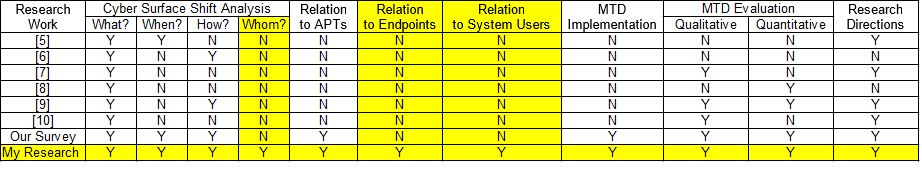
\includegraphics[width=1.3938\textwidth, height=0.5\textwidth]{2023-09-11 22 17 33.png}
            \end{figure}
        
    \subsection{Public Git Repo Link}
        \paragraph{Git Link Below}
        \hfill \break
        \href{
            https://ieeexplore.ieee.org/abstract/document/9040520
        }
            {A Survey of Privacy Protection and Network Security in User On-Demand Anonymous Communication}
            \\
        \url{https://ieeexplore.ieee.org/abstract/document/9040520}

% Last section as references
\medskip
\printbibliography
\end{document}
